\section{Results} \label{Results}

\subsection{Baseline calibration} \label{Baseline calibration}

The disaster risk model was fully calibrated except for values of $\beta$ (or $\rho$) where $\beta = \frac{1}{1+\rho}$ which was set to 0.95, corresponding to an annualized, hypothetical risk-free interest rate ``if consumption were known to be constant forever at its current level, with no growth and no volatility'' \cite{Constantinides2003} of 5\%\footnote{5\% is approximately the annual, unweighted average of nominal T-bills and bonds in \citet{Jorda2017} across countries in the sample and was also used by \citet{Weil1989} for calibration that resulted in the \textit{risk-free rate puzzle}} and the IES which was set to the value of microeconometric evidence from cross-individual differences in after-tax real interest rates of (around) 2 \cite{Gruber2013}. Table \ref{tab:growth_non_disaster} in the appendix provides additional moments used for calibration of exogeneous productivity growth and variability during non-disaster periods.

Solving the non-linear equation for the ERP incorporating disaster risk with \texttt{MINPACK}'s \texttt{hybrd} subroutine implemented in Python yielded the implied coefficients of relative risk aversion $\boldsymbol{\gamma}$. For comparison the implied coefficients of relative risk aversion from the original specification leading to the puzzle indicated with an upper bar are also presented in table \ref{tab:results_consumption} below.\\

{\renewcommand{\arraystretch}{1.0}
\begin{table}[!ht]
\begin{center}
\begin{tabular}{rccccccc}
\hline
\hline
Country & $g^{*}$ (\%) & $\rho^{*}$ & $\beta^{*}$ & $r^{e}$ (\%) & $r^{f}$ (\%) & \underline{$\gamma$} & \boldsymbol{$\gamma$}\\
\hline

Australia & 1.55 & 0.0628 & 0.9409 & 6.91 & 2.52 & 20.10 & 5.54\\ 

Belgium & 2.14 & 0.0419 & 0.9598 & 7.14 & 3.20 & 7.91 &  2.54\\ 

Denmark & 1.69 & 0.0308 & 0.9701 & 6.77 & 3.50 & 17.66 &  6.53\\ 

Finland & 2.61 & 0.0444 & 0.9575 & 7.82 & 0.92 & 34.01 &  8.15\\ 

France & 1.82 & 0.0405 & 0.9610 & 6.70 & 3.81 & 10.17 &  2.07\\ 

Germany & 2.17 & 0.0622 & 0.9415 & 7.54 & 0.56 & 34.08 &  5.13\\ 

Italy & 1.66 & 0.0310 & 0.9700 & 6.76 & 2.43 & 47.37 &  7.21\\ 

Japan & 2.65 & 0.0456 & 0.9564 & 7.20 & 1.01 & 20.62 &  0.97\\ 

Netherlands & 2.12 & 0.0429 & 0.9588 & 7.16 & 2.82 & 9.41 &  2.66\\ 

Norway & 2.09 & -0.0426 & 1.0445 & 6.96 & 3.63 & 36.28 &  12.67\\ 

Portugal & 2.79 & -0.0777 & 1.0843 & 7.25 & 4.49 & 21.17 &  8.61\\ 

Spain & 2.54 & 0.0226 & 0.9780 & 7.47 & 3.23 & 11.23 &  5.09\\ 

Sweden & 2.04 & 0.0159 & 0.9843 & 7.18 & 2.88 & 34.45 &  14.48\\ 

Switzerland & 1.69 & 0.0519 & 0.9507 & 6.94 & 3.10 & 15.88 &  6.49\\ 

United Kingdom & 1.48 & 0.0290 & 0.9718 & 6.65 & 2.69 & 76.32 &  13.36\\ 

United States & 1.98 & -0.0028 & 1.0028 & 6.98 & 2.80 & 51.76 &  11.01\\
\hline
Global & & & & & & &\\
\hline 
\hline
\end{tabular} 
\end{center}
\caption{Calibration \& results (consumption)}
\label{tab:results_consumption}
\end{table}
The results for GDP data are documented in table \ref{tab:results_GDP} in the appendix. A few observations can be made from these results:
\begin{enumerate}
    \item When accounting for disaster risk \textbf{all} implied coefficients of relative risk aversion decrease. For consumption (GDP) data the implied coefficients drop by 72\% (69\%) on average compared to the benchmark values.
    \item The relative order is approximately preserved, meaning that the disaster risk model is consistent when accounting for heterogeneity in disaster characteristics (see figure \ref{fig:disaster_vs_benchmark_gamma}).
    \item Risk-free rates are consistently overestimated. They are, nevertheless roughly in line with the levels of their empirical counterparts and this relationship is statistically significant at the 0.05 confidence level (see figures \ref{fig:actual_vs_predicted_rates_cons} and \ref{fig:actual_vs_predicted_rates_GDP} [appendix] for consumption and GDP data, respectively). However, predicted risk-free rates are upwards biased (also statistically significant mean of residuals, $\mu^{cons} = -2.54$, $\mu^{GDP} = -2.62$) and are never negative whereas long-run real T-bill rates were negative for six countries in the sample.
    \item For consumption (GDP) data two (six) countries have negative implied effective time preference rates $\rho^{*}$, meaning that $\beta^{*} > 1$ when assuming that markets are complete, i.e. $(1+r^{*})\beta^{*} = 1$ and $r^{*} = \rho^{*}$ in the steady state. From a mathematical point of view this may be problematic: the infinite, discounted sum of expected utility explodes as $t \longrightarrow \infty$. Intuitively, agents prefer present utility over utility in the future due to \textit{impatience}. This presumption translates into a positive interest rate. If this wasn't the case agents would have an incentive to borrow an infinite amount and the transversality condition would be violated which cannot coincide with a competitive equilibrium. However, \citet{Kocherlakota1990} argues that a parameterized version of the subject discount factor (such as $\beta^{*}$) greater than 1 can indeed coincide with a competitive equilibrium in a growth environment, given that a) the IES is less than 1 and the stream of consumption is constant. Under these conditions the agent prefers future consumption over present consumption which conflicts with the empirical observation that real interest rates are typically positive. In the sample presented in chapter \ref{Data}, however, seven countries appeared to have negative real T-bills rates whereas the model predicted strictly positive risk-free rates. Of those seven countries three implied negative effective time preference rates $\rho^{*}$ when using GDP data. Also, \citet{Hansen1982} derived point estimates of $\beta$ significantly greater than 1, adding support that in artificial economies ``unreasonable'' \cite{Kocherlakota1990} values for $\beta > 1$ shouldn't be precluded.
    \item In general, when moving from GDP data to consumption data four out of six countries' effective subjective discount factors $\beta^{*}$ become less than 1, indicating that consumption is a more robust measure with respect to intertemporal considerations than overall output. Effective time preference rates, however, behave inconsistently when using consumption and GDP data, meaning that for one country (Norway) $\beta^{*}$ gets closer to 1 (from GDP to consumption) whereas for the other country (Portugal) $\beta^{*}$ moves further away from 1. 
    \item The implied coefficients of relative risk aversion are somewhat higher when using GDP data compared to consumption data. Levels of the predicted rates are also higher, shifted by a constant that is due to the effect of the product of lower disaster probability and average disaster size which more than outweighs the higher average growth rates and higher variability in growth rates in non-disaster years.
\end{enumerate}

\begin{figure}[H]
	\begin{tabular}{cc}
	\subfloat[Consumption data implied $\gamma$]{
		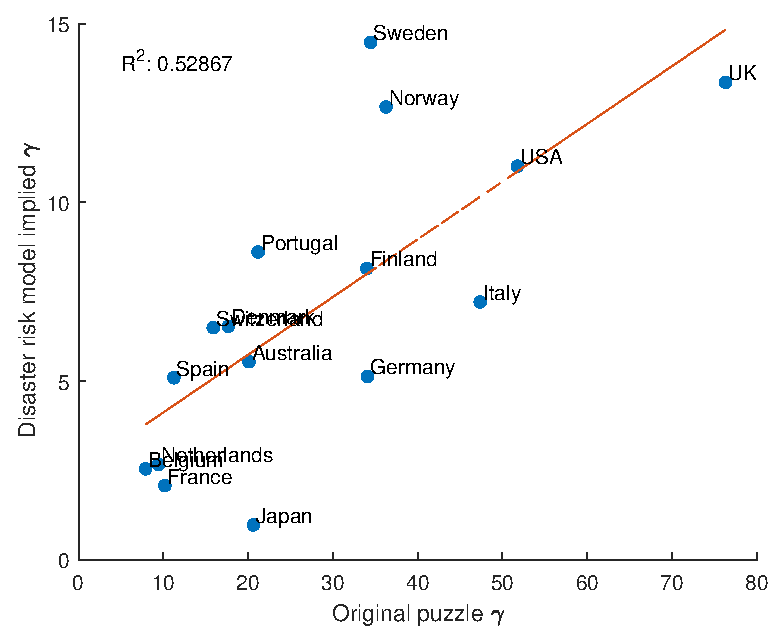
\includegraphics[width = 0.45\textwidth]{Matlab Graphics/Reduction_gamma_cons}
	} &
	\subfloat[GDP-data implied $\gamma$]{
		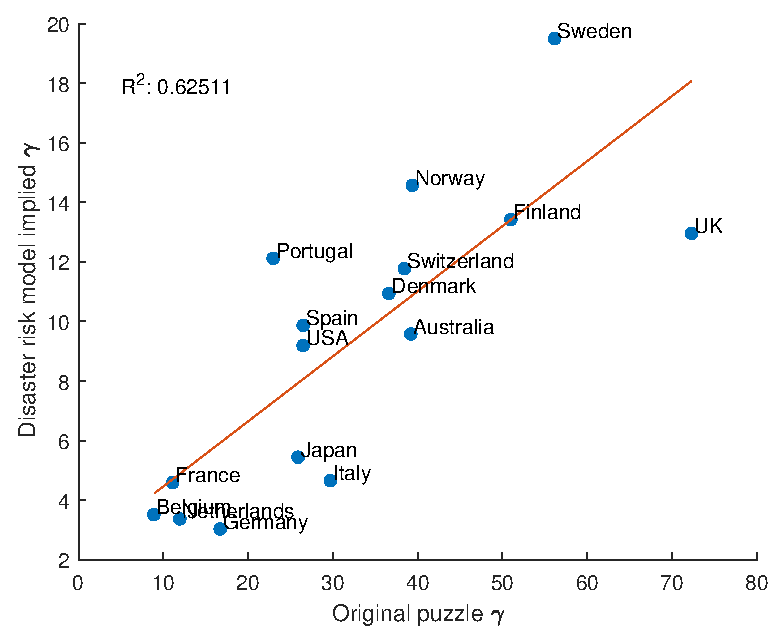
\includegraphics[width = 0.45\textwidth]{Matlab Graphics/Reduction_gamma_GDP}
	}\\
	\end{tabular}
	\caption{Disaster model $\gamma$ vs. benchmark model $\gamma$}
	\label{fig:disaster_vs_benchmark_gamma}
\end{figure}


\begin{figure}[H]
	\begin{tabular}{cc}
	\subfloat[Expected rates of return on equity]{
		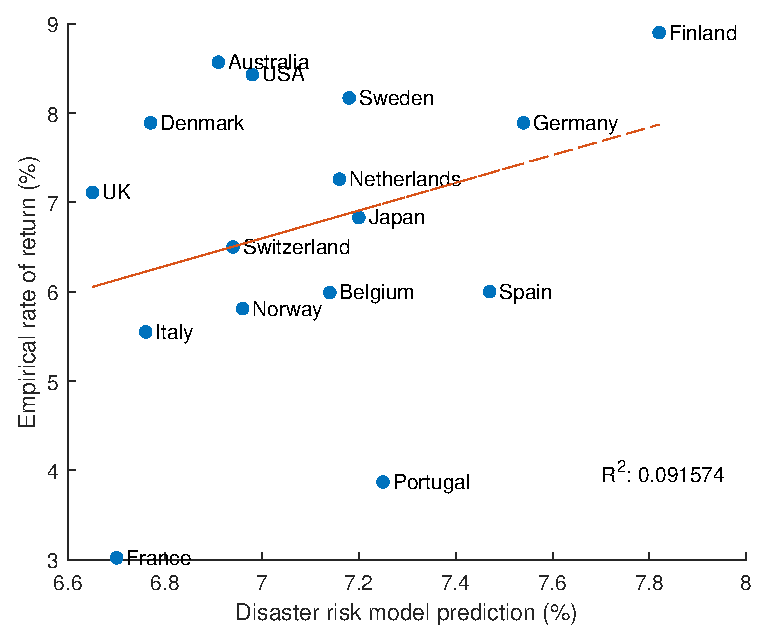
\includegraphics[width = 0.45\textwidth]{Matlab Graphics/Actual_vs_predicted_equity_cons}
	} &
	\subfloat[Risk-free rates]{
		\includegraphics[width = 0.45\textwidth]{Matlab Graphics/Actual_vs_predicted_riskfree_cons}
	}\\
	\end{tabular}
	\caption{Actual vs. predicted rates of return (consumption data)}
	\label{fig:actual_vs_predicted_rates_cons}
\end{figure}


\subsection{Robustness} \label{Robustness}

As already mentioned the disaster threshold was chosen arbitrarily, thus verifying robustness of the results when varying that parameter seems appropriate. When increasing the threshold from a proportionate decline of 9.5\% to 15\% (see table \ref{tab:disaster_risk_threshold} in the appendix) the total number of disaster events in the sample decreases from 60 to 40 and from 56 to 32 for consumption data and GDP data, respectively. 

{\renewcommand{\arraystretch}{1}
\begin{table}[p]
\begin{center}
\begin{tabular}{rccccccc}
\hline
\hline
Country & $g^{*}$ (\%) & $\rho^{*}$ & $\beta^{*}$ & $r^{e}$ (\%) & $r^{f}$ (\%) & \underline{$\gamma$} & \boldsymbol{$\gamma$}\\
\hline
\multicolumn{8}{c}{Consumption}\\
\hline

Australia & 1.55 & 0.0628 & 0.9409 & 6.91 & 2.52 & 20.10 & 5.54\\ 

Belgium & 2.08 & 0.0438 & 0.9580 & 7.07 & 3.13 & 7.91 &  2.11\\ 

Denmark & 1.67 & 0.0311 & 0.9698 & 6.75 & 3.48 & 17.66 &  6.11\\ 

Finland & 2.51 & 0.0425 & 0.9593 & 7.69 & 0.80 & 34.01 &  7.00\\ 

France & 1.82 & 0.0405 & 0.9610 & 6.70 & 3.81 & 10.17 &  2.07\\ 

Germany & 2.11 & 0.0515 & 0.9510 & 7.35 & 0.37 & 34.08 &  3.14\\ 

Italy & 1.66 & 0.0310 & 0.9700 & 6.80 & 2.43 & 47.37 &  7.21\\ 

Japan & 2.65 & 0.0456 & 0.9564 & 7.17 & 1.01 & 20.62 &  0.97\\ 

Netherlands & 2.12 & 0.0429 & 0.9588 & 7.16 & 2.82 & 9.41 &  2.66\\ 

Norway & 2.02 & -0.0358 & 1.0371 & 6.91 & 3.58 & 36.28 &  12.30\\ 

Portugal & 2.70 & -0.0564 & 1.0598 & 7.17 & 4.41 & 21.17 &  7.41\\ 

Spain & 2.31 & 0.0326 & 0.9684 & 7.33 & 3.08 & 11.23 &  4.61\\ 

Sweden & 2.04 & 0.0186 & 0.9818 & 7.18 & 2.89 & 34.45 &  15.05\\ 

Switzerland & 1.67 & 0.0532 & 0.9495 & 6.94 & 3.10 & 15.88 &  6.55\\ 

United Kingdom & 1.48 & 0.0290 & 0.9718 & 6.65 & 2.69 & 76.32 &  13.36\\ 

United States & 1.98 & -0.0028 & 1.0028 & 6.98 & 2.80 & 51.76 &  11.01\\
\hline
Global & & & & & & &\\
\hline
 & & & & & \\
  & & & & & \\
\hline
\multicolumn{8}{c}{GDP}\\
\hline
Australia & 1.71 & 0.0429 & 0.9589 & 6.92 & 2.53 & 39.18 & 9.20\\ 

Belgium & 2.30 & 0.0346 & 0.9665 & 7.25 & 3.31 & 8.88 &  3.32\\ 

Denmark & 1.84 & -0.0082 & 1.0083 & 6.74 & 3.48 & 36.61 &  9.00\\ 

Finland & 2.29 & 0.0317 & 0.9692 & 7.43 & 0.54 & 50.99 &  9.23\\ 

France & 2.14 & 0.0162 & 0.9840 & 6.96 & 4.07 & 11.10 &  4.60\\ 

Germany & 2.40 & 0.0482 & 0.9540 & 7.54 & 0.56 & 16.70 &  2.36\\ 

Italy & 2.10 & 0.0248 & 0.9758 & 7.03 & 2.70 & 29.69 &  4.65\\ 

Japan & 2.85 & 0.0250 & 0.9756 & 7.50 & 1.34 & 25.89 &  2.78\\ 

Netherlands & 2.14 & 0.0403 & 0.9612 & 7.12 & 2.78 & 11.94 &  2.70\\ 

Norway & 2.27 & -0.0919 & 1.1012 & 7.07 & 3.74 & 39.36 &  16.23\\ 

Portugal & 2.06 & -0.0400 & 1.0417 & 6.92 & 4.16 & 22.95 &  12.11\\ 

Spain & 2.14 & 0.0100 & 0.9901 & 7.05 & 2.81 & 26.49 &  6.62\\ 

Sweden & 2.18 & -0.0594 & 1.0631 & 7.14 & 2.84 & 56.16 &  18.90\\ 

Switzerland & 1.62 & 0.0348 & 0.9664 & 6.81 & 2.97 & 38.42 &  12.06\\ 

United Kingdom & 1.55 & 0.0231 & 0.9774 & 6.69 & 2.73 & 72.30 &  12.96\\ 

United States & 2.25 & 0.0056 & 0.9944 & 7.18 & 2.99 & 26.47 &  7.54\\
\hline
Global & & & & & & &\\
\hline 
\hline
\end{tabular} 
\end{center}
\caption{Calibration \& results (disaster threshold = 0.15)}
\label{tab:results_threshold}
\end{table}

Hence, overall disaster probability decreases from 2.92\% to 1.90\% and from 2.60\% to 1.44\% for consumption data and GDP data, respectively. The average disaster size, on the other hand, increases from 28.99\% to 32.69\% and from 22.23\% to 29.17\% for consumption data and GDP data, respectively.

The implied coefficients of relative risk aversion (table \ref{tab:results_threshold} below) do not change substantially or do not change at all.

Applying the Hodrick-Prescott filter\footnote{I used the Python implementation \texttt{tsa} from the \texttt{statsmodels} API which performs the method equivalent to Matlab's built-in \texttt{hpfilter} function} with $\lambda = 100$ to the annual, raw consumption expenditures and GDP indices may eliminate periods of temporary measurement error in consumption and GDP. As a result (see table \ref{tab:disaster_risk_HP}), seven (nine) countries did not experience disastrous declines in consumption (GDP) growth rates. Average duration, however, was higher compared to the raw data. The resulting volatility of consumption and GDP growth was too small after filtering, deteriorating the standard model's and the disaster risk model's ability to link asset returns and real-economy based aggregates. The implied risk aversion coefficients appear to still decrease relative to the benchmark model but some of them are 0, implying risk neutrality when derived from HP-filtered data (see table \ref{tab:results_HP} in the appendix). This robustness specification is also the only one which predicted a negative interest rate (Australia).

Varying the IES predicted a common behaviour across countries, that is the predicted rates of expected return on equity and risk-free rate decreased quickly on the interval $\psi \in (0,0.5]$ and then converge, leaving the risk premium (and coefficient of relative risk aversion) unaffected.

